\documentclass{school-22.211-notes}
\date{March 21, 2012}

\begin{document}
\maketitle

\lecture{One-Group Diffusion: Multiplying Medium} \label{1g-source}
We are going to cover some classical examples to understand the mechanics, boundary conditions, and interface conditions. Know these for the exam. 

\topic{Sphere Geometry}
\begin{enumerate}
\item For a non-multiplying medium ($\Sigma_f = 0$), and assume that $D, \Sigma_a$ are constant in space, we arrive at the \hi{inhomogeneous Helmholtz Equation}, 
\eqn{ - D \laplacian \phi (\vecr) + \Sigma_a \phi (\vecr) = S(\vecr) }
We define the diffusion length as $\displaystyle L = \sqrt{\frac{D}{\Sigma_a}}$, then the balance equation becomes, 
\eqn{ - \laplacian \phi (\vecr) + \frac{1}{L^2} \phi(\vecr) = \frac{S(\vecr)}{D} }

\item For a multiplying medium, we typically use $\displaystyle B^2 = \frac{\frac{\nu \Sigma_f}{\keff} - \Sigma_a}{D}$. 
\eqn{ - D \laplacian \phi (\vecr) + \left(\Sigma_a - \nu \Sigma_f \right) \phi (\vecr) = S(\vecr) }
\eqn{ - \laplacian \phi (\vecr) +  \frac{\Sigma_a}{D} \left( 1 - \frac{\nu \Sigma_f}{\Sigma_a} \right) \phi (\vecr) = \frac{S}{D} }

Next we are going to consider a bare sphere case:
\begin{enumerate}
\item For $\kinf < 1$, we define $\psi = \frac{\phi(r)}{r}$, and can solve the homogeneous one: 
\eqn{ \psi = C_1 e^{\kappa r} + C_2 e^{-\kappa r} }
we know that the particular solution is $\phi_p = \frac{S_0}{\left( 1 - \frac{\mu \Sigma_f}{\Sigma_a} \right) \Sigma_a}$, then 
\eqn{ \phi = \frac{C_1 e^{\kappa r}}{r} + \frac{C_2 e^{-\kappa r}}{r} +  \frac{S_0}{\left( 1 - \frac{\mu \Sigma_f}{\Sigma_a} \right) \Sigma_a} }

\item For $\kinf > 1$ and $\left( \frac{\nu \Sigma_f}{\Sigma_a} - 1 \right) > 0$, then 
\eqn{ \dpsidrn2 + \frac{\Sigma_a}{D} \left( \frac{\nu \Sigma_f}{\Sigma_a} - 1 \right) \psi(r) = 0 }
that is, $\psi(r) = C_1 \cos (B_m r) + C_2 \sin (B_m r)$. Then the solution form is, 
\eqn{ \phi(r) = \frac{C_1}{r} \cos (B_m r) + \frac{C_2}{r} \sin (B_m r) - \frac{S_0}{\nu \Sigma_f - \Sigma_a} }
BCs: 
\begin{itemize}
  \item $\phi(0)$ has to be finite. $\displaystyle \lim_{r \to 0} \frac{\sin(B_m r)}{r} = B_m, \lim_{r \to 0} \frac{\cos (B_mr)}{r} = \infty$ thus $C_1 = 0$. 
  \item $\phi(\tilde{R}) = 0$. We fine $C_2$. 
\end{itemize}
Final solution is, 
\eqn{ \phi(r) = \frac{S_0}{\nu \Sigma_f - \Sigma_a} \left[ \frac{\tilde{R}}{r} \frac{\sin (B_m r)}{\sin (B_m \tilde{R})} - 1 \right]  \label{bare-sphere} }
\hi{Notice $B_m \tilde{R} = \pi$ is where the flux becomes undefined; there is no steady-state solution; it is a critical reactor with a source}. 
\end{enumerate}

Comments:
\begin{itemize}
\item Subcritical reactor: only has a steady state solution when there is a source. 
\item Critical reactor: only has a steady state solution when there is no source. 
\end{itemize}


\item Now we consider a critical bare reactor with no source. 
\eqn{ \phi(r) = \frac{C_1}{r} \cos (B_m r) + \frac{C_2}{r} \sin (B_m r) }
Apply similar BCs, 
\begin{itemize}
  \item $\phi(0)$ has to be finite. $C_1 = 0$. 
  \item $\displaystyle  \phi(\tilde{R}) = 0 \Rightarrow \frac{C_2}{\tilde{R}} \sin (B_m \tilde{R} )$, that is, $B_m \tilde{R} = n \pi$, where $n = 1$ is the fundamental mode, others are higher modes (higher modes can be negative, not that the total flux would be negative, but that the higher mode is a negative addition to the fundamental modes). 
\end{itemize}
Comments:
\begin{itemize}
\item The fact that we cannot solve for $C_2$ implies that reactor can go critical at any power as long as we do not have any feedbacks.  
\item $B_m = B_g$ means critical; $B_m < B_g$ means subcritical; $B_m > B_g$ means super-critical. $B_m^2 = \frac{\nu \Sigma_f - \Sigma_a}{D}, B_g^2 = \left(\frac{\pi}{R} \right)^2$.  
\end{itemize}
The bigger the core is, the more oscillation there is. 

\item Fundamental mode of Helmholtz equation: we start with a bare homogeneous reactors, \hi{notice geometric buckling is a measurement of the flux curvature}
\eqn{ \laplacian \phi(r) + B_g^2 \phi(r) &= 0 & B_g^2 &= - \frac{\laplacian \phi(r)}{\phi(r)} }
Then plug into the 1 group diffusion equation, 
\begin{align}
 - D \laplacian \phi(r) + \Sigma_a \phi(r) &= \frac{1}{k} \nu \Sigma_f \phi(r) \\
- D B_g^2 + \Sigma_a &= \frac{1}{k} \nu \Sigma_f \\
k &= \frac{\nu \Sigma_f}{DB_g^2 + \Sigma_a}  \label{k-sphere}
\end{align}


\item Interpretation of cross section data: 
  \begin{enumerate}
    \item $\nu \Sigma_f < \Sigma_a$: sub-critical. Should have a source to be steady state. 
    \item $\nu \Sigma_f = \Sigma_a$. 
    \item $\nu \Sigma_f > \Sigma_a$, we can solve for the critical dimension using $B_m^2 = B_g^2$ (if $R < R^{\mathrm{critical}}$ then subcritical etc). Alternatively we can perform the fundamental mode of Helmoltz equation and get $\displaystyle k = \frac{\nu \Sigma_f}{DB_g^2 + \Sigma_a}$. 
Should have no source to be steady state critical.  
  \end{enumerate}
\eqn{ \laplacian \phi(\vecr) + B_m^2 \phi(\vecr) &= \laplacian \phi(\vecr) - \frac{1}{L^2} \phi(\vecr)= - \frac{S}{D} & B_m^2 = -\frac{1}{L^2} = \frac{\nu \Sigma_f - \Sigma_a}{D} \label{bal-eqn}}
\end{enumerate}



\clearpage
\topic{Plane Geometry}
If we solve for a plane geometry, we would get
\eqn{ \phi(x) = \left\{ \begin{array}{cc} C_n \cos (B_m x) & n = \mathrm{odd} \\ C_n \sin (B_m x) & n = \mathrm{even} \end{array} \right. }
But the only mode that is positive everywhere is $n=1$. Thus $\displaystyle B = \frac{\pi}{\tilde{L}}$. Plug $\phi(x) = \cos \left( \frac{\pi}{\tilde{L}} x \right)$ back into the balance equation, 
\begin{align}
- D \dphidxn2 + \Sigma_a \phi(x) &= \frac{1}{k} \nu \Sigma_f \phi (x) \\
D C_1  \left( \frac{\pi}{\tilde{L}} \right)^2 \cos  \left( \frac{\pi}{\tilde{L}} x \right) + \Sigma_a C_1  \left( \frac{\pi}{\tilde{L}} x \right) &= \frac{1}{k_1} \nu \Sigma_f C_1  \left( \frac{\pi}{\tilde{L}} x \right) 
\end{align}
\eqn{ k_1 &= \frac{\nu \Sigma_f}{D \left( \frac{\pi}{\tilde{L}} \right)^2  + \Sigma_a} }
which agrees with Eq.~\ref{k-sphere}, provided that $B_g^2 = \left( \frac{\pi}{\tilde{L}} \right)^2$ for a slab. Further more, the secondary mode yields an eigenvalue of, 
\eqn{ k_2 &= \frac{\nu \Sigma_f}{D  \left( \frac{2\pi}{\tilde{L}} \right)^2  + \Sigma_a} }
which leads to the discussion of 
\eqn{ \mbox{Dominance Ratio} = \frac{k_2}{k_1} = \frac{D \left( \frac{\pi}{\tilde{L}} \right)^2  + \Sigma_a}{D  \left( \frac{2\pi}{\tilde{L}} \right)^2  + \Sigma_a} }
DR is a measure of the stability. The closer it is to 1 (the larger the system is), the less stable it is (the longer it oscillates). It governs left-right/top-bottom oscillation. 


\hi{A rule of thumb about $k$}: in real reactor application, there is no source, so the balance equation is, 
\eqn{ -D \laplacian \phi + \Sigma_a \phi = \nu \Sigma_f \phi }
and the above equation describes a critical system (because in real reactor otherwise either the flux would die out or it would explode and we would have no steady state solution). However in academic reason we are interested in the subcritical and the supercritical condition as well, so we add in an artificial $k$ on the bottom of the fission term which would make the equation critical: 
\eqn{ -D \laplacian \phi + \Sigma_a \phi = \frac{\nu \Sigma_f}{k} \phi }
Notice the $k$ here is just a measurement of criticality of the system; it is not physical in the sense that a physically existing system can only have $k=1$. 



%%%%%%%%%%% 11 Spring %%%%%%%%%%%
\clearpage
\topic{Arbitrary Source in Finite Multiplying Medium} \label{one-group-source-problem-subcritical}
Consider a subcritical multiplying medium, slab geometry from $-L/2$ to $L/2$, and with a source. 
\begin{align}
  - D \dphidxn2 + \Sigma_a \phi(x) &= \nu \Sigma_f \phi(x) + S(x) \\
  \dphidxn2 + B_m^2 \phi(x) &= -\frac{S(x)}{D} 
\end{align}
Given $\Sigma_a > \nu \Sigma_f$, $B^2 = \frac{\nu \Sigma_f - \Sigma_a}{D} < 0 $, we re-write $B^2 = - |B|^2$,
\eqn{ \dphidxn2 - |B|^2 \phi(x) = \tilde{S}(x) }
The general/homogeneous solution is,
\eqn{ \phi_H (x) = A e^{|B|x} + Ce^{-|B|x} = A \cosh (|B|x) + C \sinh (|B| x) }
The particular solution depends on source $\tilde{S}(x)$. Apply BCs $\phi \left( \pm \frac{L}{2} \right) = 0$, we get the boundary conditions in the matrix form,
\eqn{ \left[ \begin{array}{cc} 
\cosh(|B|L/2) & \sinh(|B|L/2) \\
\sinh(|B|L/2) & \cosh(|B|L/2) 
\end{array} \right] 
\left[ \begin{array}{c}
A \\ C \end{array} \right] 
= - \left[ \begin{array}{c} 
\phi_p(L/2) \\ \phi_p(-L/2) \end{array} \right] }
Coefficients A and C are uniquely determined for a given source distribution: 
\begin{itemize}
\item There always exists a physically realizable solution (no critical buckling!);
\item In the limit of $S\to 0$, the only physical solution is the trivial solution. 
\end{itemize}




\clearpage
\topic{Plane Source in Finite Multiplying Medium with $\kinf < 1$}
Consider a finite multiplying medium, $\kinf < 1$, a slab geometry from $0$ to $H$, and a plane source at $0$.  
\eqn{ B_m^2 = \frac{\nu \Sigma_f - \Sigma_a}{D} &= \frac{k_{\infty} - 1}{L^2} < 0, & B_m^2 &\to -|B_m|^2}
\begin{enumerate}
\item For the homogeneous solution, we assume there is no source, 
\eqn{\dphidxn2 - |B_m|^2 \phi &= 0, &\phi(x) &= A\cosh(|B_m|x) + B \sinh(|B_m|x) }

\item BC 1: $\displaystyle \phi(0) = \phi_0, \phi(H) = 0$, we can solve for the coefficients, 
\eqn{ \boxed{\phi(x) = \phi_0 \left[ \cosh(|B_m|x) - \frac{\cosh(|B_m|H)}{\sinh(|B_m|H)} \sinh(|B_m|x) \right] } }

\item Extreme condition: if we let the size of the slab to go to infinity, 
\eqn{\lim_{H \to \infty} \phi(x) = \phi_0 [\cosh(|B_m|x) - \sinh(|B_m|x)] = \phi_0 e^{-|B_m|x} = \frac{S_0L}{2D} e^{-|B_m|x} }



\item Notice in both finite and infinite case, the fluxes have convex shapes; the finite curve is below the infinite curve though. 
\begin{figure}[ht]
  \centering
  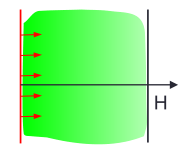
\includegraphics[width=2.5in]{images/dfs/plane-multiplying-geo.png}
  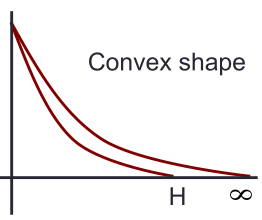
\includegraphics[width=2.5in]{images/dfs/plane-multiplying-phi.png}
  \caption{Plane Source in Finite Multiplying Medium with $\kinf < 1$}
\end{figure}
\end{enumerate}


\clearpage
\topic{Plane Source in Finite Multiplying Medium with $\kinf > 1$}
Consider a finite multiplying medium with $\kinf > 1$, it is a slab extending from $-H/2$ to $H/2$, it is subcritical with leakage, BC are from the current at center and the zero flux at the H/2 boundary. 
\eqn{ \dphidxn2 + B_m^2 \phi &= 0,  & B_m^2 &= \frac{\nu \Sigma_f - \Sigma_a}{D} = \frac{\kinf - 1}{L^2} > 0  &\phi(x) &= A \cos(B_mx) + B\sin(B_mx) }
BC1: $\phi(H/2) = 0$; BC2: $J(0) = \frac{S_0}{2}$. We can solve for the coefficients, and place absolute sign to represent the whole geometry: 
\eqn{ \phi(x) = \frac{S_0}{2DB_m \cos\left( \frac{B_m H}{2} \right)} \sin\left[ B_m \left(\frac{H}{2} - |x|\right) \right] }
Interpretations:
\begin{enumerate}
\item Because $\kinf > 1$, the flux shape is concave, that is, increasing negative slopes in the positive domain. In Fig.~\ref{approach-critical}, flux is convex when $\kinf < 1$ and concave when $\kinf > 1$, until we hit the cosine shape when $\keff = 1, \kinf = 1 + B^2L^2$ from 
  \eqn{ B^2 &= \frac{\frac{\nu \Sigma_f}{\keff} - \Sigma_a}{D} = \frac{\frac{\kinf}{\keff} - 1}{L^2}  & \kinf &= \keff + B^2 L^2}
\item If $H$ is increased to the critical dimension, that is, $H \to \frac{\pi}{B_m}$, then $\phi(0) \to \infty$; that is, if the reactor is critical, the flux at the source is infinite. That is, there is no steady-state solution for flux at the source site. In fact, if we place a fission detector at $x=0$ and measure source multiplication, 
  \eqn{M_s(0) = \frac{N_d \sigma_{f,d} V_d \phi(0)}{S_0} \propto \frac{\sigma_f}{2DB} \tan\left(\frac{BH}{2} \right) }
  Or the inverse source multiplication factor, 
  \eqn{ \frac{1}{M_s(0)} \propto \frac{1}{\tan\left(\frac{BH}{2} \right)} \to 0 }
\item To reach criticality, we can add fuel elements, withdraw control rods, and dilute boron. 1/M is useful for estimating criticality as shown in Figure~\ref{approach-critical}. 
  \begin{figure}[ht]
    \centering
    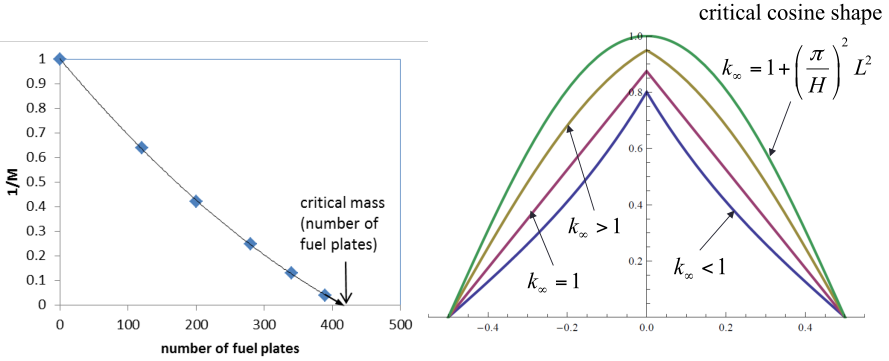
\includegraphics[width=5in]{images/dfs/approach-critical.png}
    \caption{1/M plot and Flux Shape In Approaching Criticality}\label{approach-critical}
  \end{figure}
\end{enumerate}




\clearpage
\topic{Summary}
\begin{enumerate}
\item \textbf{Super-positioning of sources}: if we are given a random source that is the sum of a couple of common forms of sources, we can super-position the flux from each of the common sources. This method works in any non-multiplying medium, and in multiplying medium in subcritical condition\footnote{Supercritical condition, as source increaes, flux inverts}. For instance, we can super-position point sources to get a line source. 

\item Diffusion theory is valid: 
  \begin{itemize}
    \item when there is little geometry heterogeneity;
    \item when $\Sigma_a \ll \Sigma_s$;
    \item when position is not too close to interface and source.
  \end{itemize}
  Diffusion theory is not valid near singularities. 

\item $\kinf$ is important\footnote{know this for the exams}: 
  \begin{itemize}
  \item $\kinf = 1$: flux is straight line;
  \item $\kinf < 1$ means $B^2 < 0$, flux is $\sinh, \cosh$ which is convex; 
  \item $\kinf > 1$ means $B^2 > 0$, flux is $\sin, \cos$ which is concave. 
  \end{itemize}
\end{enumerate}

  \begin{table}[ht]
    \centering
    \begin{tabular}{|c|c|c|c|c|} \hline
      Source & Geometry & Material &BCs & Flux \\ \hline \hline
      Point & $\infty$ Sphere & Non-multi.  & $\displaystyle \lim_{r\to\infty} \phi = 0, \lim_{r\to 0} 4 \pi r^2 J(r) = S_0$ & $\displaystyle \frac{S_0}{4\pi D} \frac{e^{-r/L}}{r}$ \\ \hline
      Plane & $\infty$ Slab & Non-multi. &$\displaystyle \lim_{x\to \infty} = 0, \lim_{x \to 0} J(x)  = \frac{S_0}{2}$ & $\displaystyle \frac{S_0 L}{2D} e^{-|x|/L}$ \\ \hline
      Plane & Finite Slab &Multi. $\kinf < 1$ & $\phi(0) = \phi_0, \phi(H) = 0$ & $\displaystyle \phi_0 \left[ \cosh(|B|x) - \coth(|B|H) \sinh(|B| x) \right]$ \\ \hline
      Plane & Finite Slab &Multi. $\kinf > 1$ & $\displaystyle \phi(H/2) = 0, J(0) = \frac{S_0}{2}$ & $\displaystyle \frac{S_0}{2D B_m \cos (BH/2)} \sin \left[ B \left( \frac{H}{2} - |x| \right) \right]$ \\ \hline
    \end{tabular}
    \caption{Subcritical System: Source and Flux} 
  \end{table}









%%%%%%% Criticality %%%%%%%%
\lecture{One-Group Diffusion: Criticality Problem} \label{1g-criticality}
In this section, we consider a critical multiplying system with no source (no source to reach steady state). 

\topic{Helmholtz Equation}
We start with the one-group diffusion equation,
\eqn{ -\divergence D(\vecr) \gradient \phi(\vecr) + \Sigma_a(\vecr) \phi(\vecr) = \frac{1}{\keff} \nu \Sigma_f(\vecr) \phi(\vecr) }
Assume homogeneous material, that is, spatial constant cross section,
\eqn{ -D \laplacian \phi(\vecr) + \Sigma_a \phi(\vecr) = \frac{1}{\keff} \nu \Sigma_f \phi(\vecr) }
Rearranging and defining a buckling term, 
\eqn{ \laplacian \phi(\vecr) + \underbrace{\frac{ \frac{\nu \Sigma_f}{\keff} - \Sigma_a}{D} }_{B^2} \phi(\vecr) = 0 }
We obtain a classic Helmholtz Equation,
\eqn{ \boxed{\laplacian \phi(\vecr) + B_m^2 \phi(\vecr) = 0 } }
Helmholtz Equation implies that,
\eqn{ B_m^2 = - \frac{\laplacian \phi(\vecr)}{\phi(\vecr)} }
Notice,
\begin{enumerate}
\item Since $B_m^2$ is a constant, that is to say $\frac{\laplacian \phi(\vecr)}{\phi(\vecr)}$ is a constant, that is to say $\phi(\vecr)$ has a constant curvature. 
\item Material buckling: 
  \eqn{ B_m^2 = \frac{\frac{\nu \Sigma_f}{\keff} - \Sigma_a}{D} }
  which matches geometry buckling, 
  \eqn{ \keff = \frac{\nu \Sigma_f}{DB_g^2 + \Sigma_a} }
  where $DB^2_g$ is the leakage per unit volume per unit flux. Notice $\keff$ does not depend on volume or flux. 

\item Critical buckling: when a system is critical, the material buckling is uniquely determined by cross sections, 
  \eqn{ B_m^2 = \frac{\nu \Sigma_f - \Sigma_a}{D} = \frac{\frac{\nu \Sigma_f}{\Sigma_a} - 1}{\frac{D}{\Sigma_a}} = \frac{\kinf - 1}{M^2} }
  \hi{Migration area} $M^2 = \frac{D}{\Sigma_a}$ is a measurement of the amount of travelling before absorption. $M^2$ is typically used in one group theory, whereas in other times we use \hi{Diffusion are $L^2$}, and it is used to measure the mean of the square of the crow-fly distance travelled by a neutron from emission to absorption respectively from the projection of the path on the x-y plane and the x-axis: 
  \eqn{    \expect{r^2} &= 6 L^2 & \expect{\rho^2} &= 4 L^2 & \expect{x^2} &= 2 L^2 }

\item Solutions exist only for certain values of the buckling such that the flux is everywhere positive and vanishing on outer (or extrapolated) surfaces; we define these unique values as `geometrical buckling' $B_g^2$. The allowable values of geometrical buckling that satisfy the boundary conditions are uniquely determined reactor geometry.

\item For a criticality problem, we can solve find the $B^2$ such that the system is critical. Hence giving geometry, only certain materials would make the system critical; given material, only certain geometries would make the system critical. That is, given a reactor, it would be critical if and only if the material and the geometry satisfy,
  \eqn{ B_g^2 = B_m^2} 

\item Solution only exists when $\kinf > 1$ (exception: if there is external source, $\kinf$ can be less than 1 and the system is still critical). 
\end{enumerate}

Talbe~\ref{simple-geometry-laplacian} lists a couple of one group homogeneous geometry Laplacians. 
\begin{table}
  \centering
  \begin{tabular}{|l|l|} \hline
    Slab & $\dphidxn2 + B^2 \phi(x) = 0$ \\ \hline
    Sphere & $\dphidrn2 + \frac{2}{r} \dphidr + B^2 \phi(r) = 0$ \\ \hline
    Infinite Cylinder & $\dphidrn2 + \frac{1}{r} \dphidr + B^2 \phi(r) = 0$ \\ \hline
    Finite Cylinder & $\dphidrn2 + \frac{1}{r} \dphidr + \dphidzn2 + B^2 \phi(r,z) = 0$ \\ \hline
    Cartesian & $\dphidxn2 + \dphidyn2 + \dphidzn2 + B^2 \phi(x,y,z) = 0$ \\ \hline
  \end{tabular}
\caption{Simple Geometry Laplacians} \label{simple-geometry-laplacian}
\end{table}




\clearpage
\topic{Critical 1D Slab}
 Consider a 1D slab $\in  \left[- \frac{L_0}{2}, \frac{L_0}{2} \right]$:
  \eqn{ \dphidxn2 + B^2 \phi (x) &= 0, &\phi(x) &= A \cos (Bx) + C \sin(Bx) }
BCs: $\phi(\pm L/2) = 0$, $\frac{L}{2} = \frac{L_0}{2} + 0.711 \lambda_{tr}$. Two equations two unknowns, 
  \eqn{ \left[ \begin{array}{cc} \cos(BL/2) & \sin(BL/2) \\ \cos(BL/2) & -\sin(BL/2) \end{array} \right] \left[ \begin{array}{cc} A \\ C \end{array} \right] = 0 }
  Set the determinant to be zero, we get $-2 \cos (BL/2) \sin (BL/2) = 0$. There are two possibilities: 
\eqn{ B_n&= \frac{n\pi}{L}  & \phi(x) &= \left\{ 
  \begin{array}{cc} 
    A_n \cos (B_n x) & n=1,3,5, \cdots \\
    A_n \sin (B_n x) & n=2,4,6, \cdots 
  \end{array} \right. }
But in order for $\phi(x) \ge 0$ everywhere, only $n=1$ is possible; that is, 
\eqn{ \phi(x) = A \cos \frac{\pi x}{L} }
and the criticality condition implies that, 
\eqn{ \frac{\nu \Sigma_f - \Sigma_a}{D}  = \left( \frac{\pi}{L} \right)^2 }

\clearpage
\topic{Critical Finite Cube}
Consider a finite cube with the dimensions $-a/2 \le x \le a/2, -b/2 \le y \le b/2, -c/2 \le z \le c/2$. The Helmholtz equation is,
\eqn{ \pphipxn2 + \pphipyn2 + \pphipzn2 + B^2 \phi = 0}
Assume separation of variables,
\eqn{ \phi(x,y,z) = X(x) Y(y) Z(z) }
\eqn{ \dXdxn2 + B_x^2 X &= 0, &\dYdyn2 + B_y^2 Y &= 0, &\dZdzn2 + B_z^2 Z &=0}
The solution is, 
\eqn{ \phi &= A \cos \left( \frac{\pi x}{L_x} \right)\cos \left( \frac{\pi y}{L_y} \right)\cos \left( \frac{\pi z}{L_z} \right) ,  &B^2 &= \left(\frac{\pi}{a}\right)^2 + \left(\frac{\pi}{b}\right)^2 + \left(\frac{\pi}{c}\right)^2 }

\clearpage
\topic{Critical Finite Cylinder} 
Consider a finite cylinder from $-H/2$ to $H/2$ with radius $R$. We assume azmimuthal symmetry of Helmholtz Equation, 
\eqn{\frac{1}{r} \ddr \left( r \pphipr\right) + \pphipzn2 + B^2 \phi = 0 }
Assume separation of variables,
\eqn{ \phi(r,z) = R(r) Z(z) }
We plut the sepration of variables into the Helmholtz Equation, break $B^2 = B_r^2 + B_z^2$, and we get two equations one for each direction, 
\eqn{ \frac{1}{R} \left( \dRdrn2 + \frac{1}{r} \dRdr \right) + B_r^2 = 0 }
\eqn{ \dZdzn2 + B_z^2 Z = 0 }
In $r$ direction, we can consider an infinite cylinder, 
\eqn{ R(r) &= A_1 J_0 (B_r r), & B_r&= \frac{2.405}{R} }
In $z$ direction, we can consider an infinite slab,
\eqn{ Z(z) &= A_2 \cos(B_z z), & B_z &= \frac{\pi}{H} } 
We combine the two directions,
\eqn{ \phi(r,z) &= A J_0 \left( \frac{2.405}{R} r\right) \cos \left( \frac{\pi z}{H} \right), &B^2 &= B_r^2 + B_z^2 = \left( \frac{2.405}{R} \right)^2 + \left( \frac{\pi}{H} \right)^2 }
Problems with less than one direction that is non-homogeneous can be solved this way with separation of variables.

\clearpage
\topic{Critical Reflected Slab Reactor}\label{critical-reflected-slab}
Consider a critical reflected slab reactor as in Figure~\ref{reflected-slab}. 
\begin{figure}[ht]
  \centering
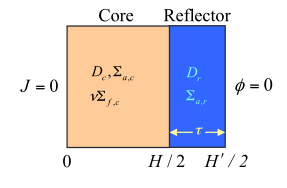
\includegraphics[width=2.5in]{images/dfs/reflected-slab.png}
\caption{A Critical Reflected Slab Geometry} \label{reflected-slab}
\end{figure}
The Helmholtz equations for the two regions are,
\eqn{-D^c \laplace \phi^c + \Sigma_a^c \phi^c &= \frac{1}{\keff} \nu \Sigma_f^c \phi^c,  &-D^r \laplace \phi^r + \Sigma_a^r \phi^r &= 0 }
\eqn{ B^2 &= \frac{\frac{\kinf}{\keff} - 1}{L_c^2}, & \kappa^2 &= \frac{1}{L_r^2} = \frac{\Sigma_a^r}{D^r} = -B_{m,r}^2 }
\eqn{ \laplace \phi^c + B^2 \phi^c &= 0, &\laplace \phi^r - \kappa^2 \phi^r &= 0}
The solutions are in the forms of,
\eqn{ \phi^c(x) &= C_1 \cos(Bx) + C_2 \sin(Bx), &\phi^r(x) &= C_3 \cosh(\kappa x) + C_4 \sinh (\kappa x) }
BC1: reflective boudnary condition at $x=0$, BC2: zero flux at reflector surface, 
\eqn{ J^c(0) &= 0 \Rightarrow C_2 = 0, & \phi(H'/2) &= 0 \Rightarrow C_3 = 0} 
We have: 
\eqn{ \phi^c (x) &= C_1 \cos (Bx), & \phi^r (x) &= C_4' \sinh[\kappa(H'/2 - x)] }
Apply two interface conditions: 
\eqn{ \phi^c (H/2) &= \phi^r (H/2), & J^c(H/2) &= J^r (H/2) }
which can be written in the matrix form, 
\begin{align}
\left[ \begin{array}{cc}
\cos (BH/2) & -\sinh(\kappa \tau) \\
D^c B \sin(BH/2) & -D^r \kappa \cosh(\kappa \tau) 
\end{array} \right] 
\left[ \begin{array}{c} 
C_1 \\ C_4' \end{array} \right] = 0
\end{align}
We define the reflector thickness $\tau = \frac{H' - H}{2}$, then the coefficients can be solved,
\eqn{ C_1 &= \phi^c (0), & C_4' &= C_1 \frac{\cos (BH/2)}{\sinh(\kappa \tau) } }
which gives us the criticality condition,
\eqn{ D^c B \tan \left(\frac{B H}{2} \right) = D^r \kappa \coth (\kappa \tau) }
Interpretation:
\begin{enumerate}
\item Since $B$ is defined with $\keff$, 
  \eqn{ B^2 = \frac{\frac{\kinf}{\keff} - 1}{L^2} }
  we need to satisty an expression between $\keff$ and $H$. We can either,
  \begin{enumerate}
  \item Given $H$, search for the $\keff$ that satisfies the equivalence;
  \item Given $\keff$, search for the $H$ that satisfies the equivalence,
    \eqn{H = \frac{2}{B_m} \tan^{-1} \left[ \frac{D^r \kappa}{D^c B_m} \coth (\kappa \tau) \right] }
    That is, as $H \down, \tau \up$. For large $\tau$, like $\kappa \tau > 3, \coth (\kappa \tau) \to 1$, the smallest $H$ to reach criticality is,
    \eqn{H = \frac{2}{B_m} \tan^{-1} \left[ \frac{D^r \kappa}{D^c B_m} \right] }
  \end{enumerate}
\item Critical dimension is reduced by the presence of the reflector: 
\eqn{   s = \frac{\tilde{H}}{2} - \frac{H}{2}   = \frac{1}{B_m} \left\{ \frac{\pi}{2} - \tan^{-1} \left[ \frac{D^r \kappa}{D^c B_m} \coth(\kappa \tau) \right] \right\} }
\eqn{   \tan\left[ \frac{\pi}{2} - \tan^{-1} x \right] &= \cot [\tan^{-1} x ] = \frac{1}{\tan[\tan^{-1} x]} = \frac{1}{x}, & \frac{\pi}{2} - \tan^{-1} x &= \tan^{-1} \left( \frac{1}{x} \right) }
\eqn{  \Aboxed{ s &= \frac{1}{B_m} \tan^{-1} \left[ \frac{D^c B_m}{D^r \kappa} \tanh(\kappa \tau) \right] } }
\item For larger cores, $B_m \to 0$ and $\tan^{-1} x \approx x $, that is, 
\eqn{ s = \frac{D^c}{D^r \kappa} \tanh(\kappa \tau) = \frac{D^c}{D^r} L^r \tanh\left( \frac{\tau}{L^r} \right)  }
That is, 
\begin{align}
  \left\{ \begin{array}{ccc} 
    \tau \ll L^r & s \approx \frac{D^c}{D^r} \tau &  (\tanh x \approx x \mbox{ for }x\ll 1) \\
    \tau \gg L^r & s \approx \frac{D^c}{D^r} L^r &  (\tanh x \approx 1 \mbox{ for }x > 3) 
  \end{array} \right. 
\end{align}
\item For more on reflector saving, see Reuss' Section 6.1.5 (p.173). 
\end{enumerate}


\clearpage
\topic{Summary}
\begin{table}[ht]
  \small
  \makebox[\textwidth][c]{
  \begin{tabular}{|l|l|l|l|} \hline
    Geometry & Diffusion Equation & Flux & Geometrical Buckling \\ \hline
    Slab $\in  \left[- \frac{L}{2}, \frac{L}{2} \right]$ &$\dphidxn2 + B^2 \phi = 0$ & $\phi = A \cos \left( \frac{\pi x}{L} \right)$ & $B^2 = \left( \frac{\pi}{L} \right)^2$ \\ 
    Sphere $\in [0, R]$  & $\dphidrn2 + \frac{2}{r} \dphidr + B^2 \phi = 0$& $\phi= \frac{A}{r} \sin \left( \frac{\pi r}{R} \right)$ & $B^2 = \left( \frac{\pi}{R} \right)^2$ \\
    Cylinder ($z: \infty$) & $\dphidrn2 + \frac{1}{r} \dphidr + B^2 \phi = 0$ & $\phi = A J_0 \left( \frac{2.405 r}{R} \right)$ & $B^2 = \left( \frac{2.405}{R} \right)^2$ \\ 
    Cylinder (z: $\pm H/2$) & $\dphidrn2 + \frac{1}{r} \dphidr + \dphidzn2 + B^2 \phi = 0$ & $\phi = A J_0\left( \frac{2.405 r}{R} \right) \cos \left( \frac{\pi z}{H} \right)$ & $B^2 = \left( \frac{2.405}{R} \right)^2 + \left( \frac{\pi}{H} \right)^2$ \\ 
    Parallelepiped ($\pm \frac{L_i}{2}$) & $\dphidxn2 + \dphidyn2 + \dphidzn2 + B^2 \phi = 0$ & $\phi = A \cos \left( \frac{\pi x}{L_x} \right) \cos \left( \frac{\pi y}{L_y} \right) \cos \left( \frac{\pi x}{L_z} \right)$ & $B^2 = \left( \frac{\pi}{L_x} \right)^2 + \left( \frac{\pi}{L_y} \right)^2 + \left( \frac{\pi}{L_z} \right)^2$ \\ \hline
  \end{tabular}
}
  \caption{One Group Fundamental Mode Eigenvalues and Eigenvectors} \label{eigen-values}
\end{table}
\normalsize

Observations:
\begin{itemize}
\item The lowest node is the only one remains after the source is gone. 
\item For any positive value of materials buckling, there is a unique critical size for each reactor geometry. 
\item Know how to get the critical buckling for different geometries. 
\item Seperation of variables works as long as there is no one more than one direction that is heterogeneous. 
\item Example: know how to find height-to-diameter to minimize leakage. The optimal cylinder has a H/D of around 0.92. 
\end{itemize}
 
  
\end{document}
